\chapter{Testing Post Development}
\label{chap:testPostDev}
Once I have finished programming my game, I will need to test all the elements of the app to ensure that I have (a) correctly programmed it, (b) there are no bugs, (c) the game meets my success criteria.

\section{Final Test Plan}

\begin{longtable}{p{0.05\textwidth}|p{0.15\textwidth}|p{0.2\textwidth}|p{0.2\textwidth}|p{0.2\textwidth}|p{0.05\textwidth}}
\textbf{Test $N\textsuperscript{\underline{o}}$} & \textbf{Test Title} & \textbf{Details} & \textbf{Expected Outcome} & \textbf{Final Outcome} & \textbf{Vid $N\textsuperscript{\underline{o}}$} \\
\hline
\endhead
1a & Loading the main menu & Start the application and wait for the first form to load. & The main menu is the first form to load. & The main menu is the first form to load. \tempText{Green}{Pass} & 1a \\
\hline
1b & Main menu buttons test 1 & From the main menu, press the 'New Game' button. & The main menu form closes and the new game creation tool form opens. & The main menu form closes and the new game creation tool form opens. \tempText{Green}{Pass} & 1b \\
\hline
1c & Main menu buttons test 2 & From the main menu, press the 'Show saved games' button. & The main menu form closes and the show saved games form opens. & The main menu form closes and the show saved games form opens. \tempText{Green}{Pass} & 1c \\
\hline
1d & Main menu buttons test 3 & From the main menu, press the 'Settings' button. & The main menu form closes and the settings form opens. & The button clicks but nothing happens as there is no settings form. \tempText{Red}{Fail} & 1d \\
\hline
1e & Main menu buttons test 4 & From the main menu, press the 'About' button. & The main menu form closes and the about form opens. & The main menu form closes and the about form opens. \tempText{Green}{Pass} & 1e \\
\hline
1f & Main menu accessibility test pt.1 & From the main menu form, maximise the window using the Windows Menu Bar. & All controls on the form will increase in size and increase the spacing between them. & All controls on the form will increase in size and increase the spacing between them. \tempText{Green}{Pass} & 1f \\
\hline
1g & Main menu accessibility test pt.2 & From the main menu form, restore down the window using the Windows Menu bar. & The controls on the form should respond by shrinking and keeping their spacing according to the new size of the window & The controls on the form should respond by shrinking and keeping their spacing according to the new size of the window \tempText{Green}{Pass} & 1g \\
\hline
2a & Generating new game with correct data & Create a new game, entering valid data and setting the save location. Then click the save button. & The app displays the main game screen form with the correct main character information displayed. & The app progresses to the main game screen. \tempText{Green}{Pass} & 2a \\
\hline
2b & Generating new game with some incorrect data & Create a new game, entering the wrong data types into the text boxes and setting the save location. For example, entering “123” into the first name field. & The app progresses as normal; numbers for names are valid entry. & The app progresses to the main game screen. \tempText{Green}{Pass} & 2b \\
\hline
2c & Generating new game leaving text boxes blank & Create a new game, without entering and information into any of the text boxes except save location. & The app will reject the input and instruct the player to enter the information or press the random button. & The app progresses to the main game screen. \tempText{Red}{Fail} & 2c \\
\hline
2d & Random generation & Create a new game and use the random button and setting the save location. & The app populates all the fields on the form with random data and then progresses onto the main game screen form. & The app populates all the fields on the form with random data and then progresses onto the main game screen form. \tempText{Green}{Pass} & 2d \\
\hline
2e & Re-roll random generation & Create a new game and use the random generation button, then press it again and setting the save location. & The app will generate two different sets of random information and display them sequentially. They should be different. The app will then progress onto the main game screen. & The app will generate two different sets of random information and display them sequentially. They should be different. The app then progresses onto the main game screen. \tempText{Green}{Pass} & 2e \\
\hline
2f & New game form accessibility & Move between the controls without using mouse. & Click in the first textbox then navigate through the form by using keyboard only. & Had to click in first textbox to enter the tab chain. Was able to move between character information successfully, however unable to move into save location or select the save button so had to use mouse. \tempText{Red}{Fail} & 2f \\
\hline
2g & New game form accessibility pt.2 & From the main menu form, maximise the window using the Windows Menu Bar. & All the controls on the form should respond by growing and keeping their spacing according to the size of the window. & Some of the controls resized, however the majority didn't. \tempText{Red}{Fail} & 2g \\
\hline
2h & New game form accessibility pt.3 & From the main menu form, restore down the window using the Windows Menu bar. & The controls on the form should respond by shrinking and keeping their spacing according to the new size of the window & All controls responded by shrinking and sorting their spacing according to the new size of the window. \tempText{Green}{Pass} & 2h \\
\hline
2i & Not specifying a save location & Generate a random game and click save without specifying a save location & The game rejects the input and displays a message box instructing users to select a save location. & The game rejects the input and displays a message box instructing users to select a save location. \tempText{Green}{Pass} & 2i \\
\hline
3a & Loading from file with correct file placement & Load the game from the a folder with all the files intact and correctly placed. & The app will load the data then display the main game screen. & The app behaves as expected and opens the correct data. \tempText{Green}{Pass} & 3a \\
\hline
3b & Loading from file with missing files & Load the game from a folder with missing files. & The app will say that files are missing and not load the game. It will clear the form ready for the next attempt. & The app crashes and displays a runtime error. \tempText{Red}{Fail} & 3b \\
\hline
3c & Loading from file with a completely wrong folder & Load the game from a random folder that doesn’t contain any of the correct files. & The app will say that files are missing and not load the game. It will clear the form ready for the next attempt. & The app crashes and displays a runtime error. \tempText{Red}{Fail} & 3c \\
\hline
3d & Show saved games form accessibility test pt.1 & From the main menu form, maximise the window using the Windows Menu Bar. & All the controls on the form should respond by growing and keeping their spacing according to the size of the window. & Some of the controls resized, however the majority didn't. \tempText{Red}{Fail} & 3d \\
\hline
3e & Show saved games form accessibility test pt.2 & From the main menu form, restore down the window using the Windows Menu bar. & The controls on the form should respond by shrinking and keeping their spacing according to the new size of the window. & All controls responded by shrinking and sorting their spacing according to the new size of the window. \tempText{Green}{Pass} & 3e \\
\hline
4a & Pressing the save and home button & From the main game screen, press the save and home button. & The app will save the data to the files then close the main game screen form and open the main menu form. & The app saved the data to the files then close the main game screen form and open the main menu form. \tempText{Green}{Pass} & 4a \\
\hline
4b & Pressing the 'age up' button & Click the age up button. & The age up algorithm is followed correctly; with no unnecessary alerts to the player. The scores should also be re-calculated and their displays updated. & The age up algorithm is followed correctly. No unnecessary alerts are displayed to the user. The score displays change. \tempText{Green}{Pass} & 4b \\
\hline
4c & Changing tabs & Using the tab menu bar control, click from tab to tab. & When clicking from tab-to-tab, the correct controls only should be displayed. & When clicking from tab-to-tab, the correct controls only should be displayed. \tempText{Green}{Pass} & 4c \\
\hline
4d & Main game screen accessibility test pt.1 & From the main game screen form, maximise the window using the Windows Menu Bar. & All the controls on the form should respond by growing and keeping their spacing according to the size of the window & The controls on the form do nothing. \tempText{Red}{Fail} & 4d \\
\hline
4e & Main game screen accessibility test pt.2 & From the main game screen form, restore down the window using the Windows Menu bar. & The controls on the form should respond by shrinking and keeping their spacing according to the new size of the window & All controls responded by shrinking and sorting their spacing according to the new size of the window. \tempText{Green}{Pass} & 4e \\
\hline
5a & Family tab - alive select & From the family tab, select an alive family member. & The family member information populates accordingly with 'N/A' for reason and date of death. & The family member information populates accordingly with 'N/A' for reason and date of death. \tempText{Green}{Pass} & 5a \\
\hline
5b & Family tab - select dead & From the family tab, select a dead family member. & The family member information populates accordingly with correct reason and date of death & The family member information populates accordingly with correct reason and date of death. \tempText{Green}{Pass} & 5b \\
\hline
6a & Choice box & Play though the game which will trigger the choice box to appear in time with education events. & The choice box appears at the correct times throughout the game with the correct information on it. & The choice box appears at the correct times throughout the game with the correct information on it. \tempText{Green}{Pass} & 6a \\
\hline
6b & Education events are visible in the correct places & After entering the age bracket where education events are generated, the education events should appear both in the main event box and in the education specific box & The education events will appear in the main event box and in the education specific event box & The education events appear in the main event box and in the education specific event box. \tempText{Green}{Pass} & 6b \\
\hline
6c & Education information is correct on the form & Before pressing age up, observe the education information and observe again after pressing age up & The education information (points, current situation) are correct on the form & The education information (points, current situation) are correct on the form. \tempText{Green}{Pass} & 6c \\
\hline
6d & Permanently withdraw from education button prevents any more education events from being generated & Press the 'Permanently Withdraw From Education' button & No more education events will generate & No more education related events get generated. \tempText{Green}{Pass} & 6d \\
\hline
7a & Commit random crime button & Press the 'Commit random crime' button & A random crime will be generated and displayed & A random crime is generated and displayed. \tempText{Green}{Pass} & 7a \\
\hline
7b & Crime event box showing the correct data only & After pressing commit random crime button, observe the crime event box & Only crime events are displayed in the crime event box. & Only crime events are displayed in the crime event box. \tempText{Green}{Pass} & 7b \\
\hline
8a & Edit character unlocks correctly & Before the main character is 13, the edit character options should be 'locked' and after they turn 13, they should be 'unlocked' & After main character turns 13, the edit character options unlock & After main character turns 13, the edit character options unlock. \tempText{Green}{Pass} & 8a \\
\hline
8b & Edit character saves data when correct data is entered & Enter correct data into the edit character options, then press save. & The main game tab should update accordingly & The main game tab updates accordingly. \tempText{Green}{Pass} & 8b \\
\hline
8c & Edit character rejects erroneous data & Empty one of the textbox controls on the edit character options, then press save & The game rejects the input. & The game rejects the input. \tempText{Green}{Pass} & 8c \\
\hline
8d & end life works as expected press yes & Press the end life button then press 'yes' on the dialogue box & The game should trigger the end life algorithm and 'kill' the main character & The game triggers the end life algorithms and 'kills' the main character. \tempText{Green}{Pass} & 8d \\
\hline
8e & end life works as expected. press no & Press the end life button then press 'no' on the dialogue box & The game should return to the edit character screen. & The game returns to the edit character screen. \tempText{Green}{Pass} & 8e \\
\hline
9a & Refresh available jobs once & Press the 'Refresh available jobs' button & The game should generate a new set of jobs. & The game generates a new set of jobs. \tempText{Green}{Pass} & 9a \\
\hline
9b & Refresh available jobs twice & Press the 'Refresh available jobs' button twice & The game should generate two different sets of jobs. & The game generates two different sets of jobs. \tempText{Green}{Pass} & 9b \\
\hline
9c & Select an available job and apply & Highlight an available job and press the 'apply' button & The game should set the current job information to the job which has just been applied for and should generate a suitable event. & The game sets the current job information to the job which has just been applied for and generates a suitable event. \tempText{Green}{Pass} & 9c \\
\hline
9d & Quit job & Press the quit job button & The game should clear the current job information. & The game clears the current job information. \tempText{Green}{Pass} & 9d \\
\hline
9e & Apply for a new job while main character currently has one & Select and apply for a job while the main character currently has one & The game should reject this and display a message box to the player saying they need to quit their current job first. & The game allows the main character to apply for a job without quitting their current one first. \tempText{Red}{Fail} & 9e \\
\hline
10a & Generate one set of potential partners & From the partners screen, press 'Generate more partners' button & The game should generate a new set of potential partners & The game generates a new set of potential partners. \tempText{Green}{Pass} & 10a \\
\hline
10b & Generate two sets of potential partners & From the partners screen, press 'Generate more partners' button twice & The game should generate two different sets of potential partners. & The game generates two different sets of potential partners. \tempText{Green}{Pass} & 10b \\
\hline
10c & Select a potential partner and take on date & From the partners screen, select a potential partner and take press take on date & The game should populate the current partner information and generate an event. & The game populates the current partner information and generates an event. \tempText{Green}{Pass} & 10c \\
\hline
10d & Dump the partner & When you have a partner, press the 'dump' button & The game should clear the current partner information. & The game clears the current partner information. \tempText{Green}{Pass} & 10d \\
\hline
11a & Generating partners after changing main characters gender and/or sexuality & After changing the main characters gender and/or sexuality, press the generate more partners button & The game should  generate the correct potential partners for the main characters new gender and/or sexuality & The game generates the correct potential partners for the main characters new gender and/or sexuality. \tempText{Green}{Pass} & 11a \\
\hline
12a & Death & Play through the game and wait for death to occur. & The game should randomly kill all people in the game. Family members should have an event generated and the main character should have a message box displayed to the player & The game randomly kills people in the game and displays it appropriately. \tempText{Green}{Pass} & FL1; FL2 \\
\hline
\end{longtable}
\textit{NB: The saved game data from video FL2 is available in the Appendix \ref{chap:exampleSaveD}}

\begin{multicols}{2}
[
\section{User Acceptance Testing}
For the final testing for my project, I will ask some of my friends \& classmates who fit into the stakeholders category to test my project and give me feedback. Their findings are listed below and will be discussed in the Evaluation chapter.
\subsection{Findings from User Acceptance Testing}
]
\textbf{Liked:}
\begin{itemize}
    \item reasons for death
    \item the changes in lengths of life
    \item the random generation of names
    \item the random generation of crimes
    \item the random generation of jobs
    \item the silly death reasons
    \item \verb|TAB| key working to move between controls on character creation form
\end{itemize}

\textbf{Didn't like:}
\begin{itemize}
    \item that the same death could occur twice in the same game
    \item the death frequency
    \item the age gap possibilities between the partner and main character
    \item when main character died at age 1
    \item even if both the parents have died, the school events reference them
\end{itemize}
\textbf{Suggested Improvements:}
\begin{itemize}
    \item buttons need labels as well as icons
    \item make the label controls on the choice box clickable too
    \item neaten the 'Save \& Home' icon so they don't overlap
    \item the main character should automatically get a job when the turn 18
\end{itemize}
\end{multicols}

\begin{multicols}{2}
[
\subsection{Observations from User Acceptance Testing}
These are observations I made while watching other people play my game:
]
\begin{itemize}
    \item Quit band 1 jobs quite frequently
    \item Didn't attempt to edit the character
    \item Didn't say but inferred liked progress bars for score display
    \item Flicked between tabs lots
    \item Users struggled with using the app without any guidance or input from me
    \item Users stayed on the main page mostly, not interacting with other elements of the game
\end{itemize}
\end{multicols}
\subsection{Evidence of my testers testing}
Shown below are screenshots of direct messages with my testers, evidencing that they were involved in the user acceptance testing.

\begin{figure}[H]
    \begin{minipage}{0.45\textwidth}
        \begin{figure}[H]
        \centering
        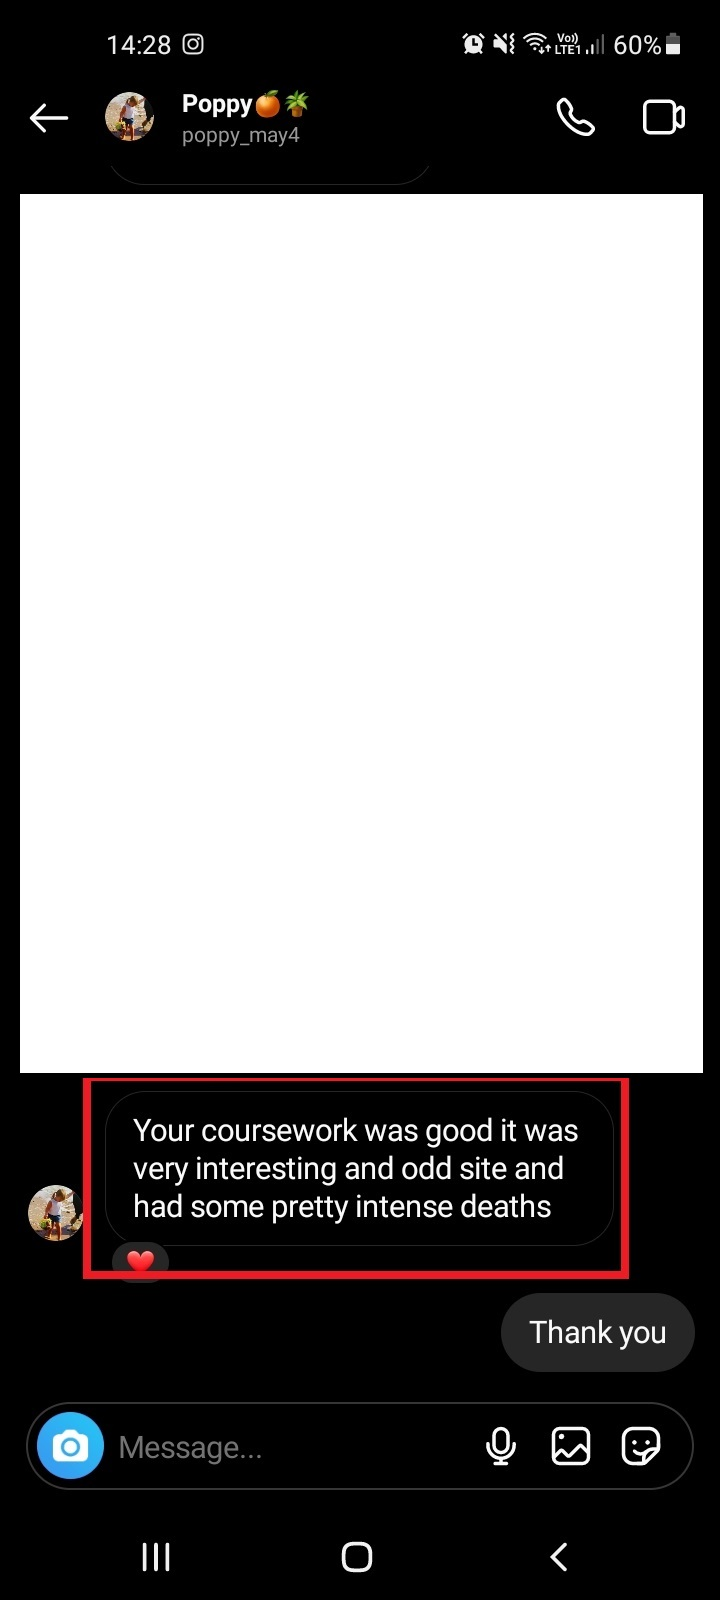
\includegraphics[width=0.9\textwidth]{images/evalutation/Evidence from Poppy.jpg}
        \caption{Evidence of tester 1 - Poppy}
        \label{fig:evidencePoppy}
        \end{figure}
    \end{minipage} \hfill
    \begin{minipage}{0.45\textwidth}
        \begin{figure}[H]
        \centering
        
\includegraphics[width=0.9\textwidth]{images/evalutation/Evidence from Nuala.jpg}
        \caption{Evidence of tester 1 - Nuala}
        \label{fig:evidenceNuala}
        \end{figure}
    \end{minipage}
\end{figure}
